\documentclass[12pt]{article}
\usepackage{changepage,soul,graphicx,graphbox,stoversymb}%,afterpage}
\usepackage[left=0.5in,right=0.5in,bottom=1in,top=0.75in]{geometry}%,showframe=true
\everymath{\displaystyle}

\usepackage{multicol}
\usepackage[many]{tcolorbox}
\usepackage[inline]{enumitem}
\usepackage{amsmath,amsthm}
	\theoremstyle{definition}
	\newtheorem{defn}{Definition}
	
	\newtheoremstyle{underl}{4.5mm}{4.5mm}{}{}{}{\textnormal{.}}{ }{\underline{\thmname{#1}}}
	\theoremstyle{underl}
	\newtheorem*{ex}{Ex}

\thispagestyle{empty}

\newenvironment{mypmatrix}[1]{\renewcommand{\arraystretch}{#1}\begin{pmatrix}}{\end{pmatrix}}
\newenvironment{mybmatrix}[1]{\renewcommand{\arraystretch}{#1}\begin{bmatrix}}{\end{bmatrix}}
\newcommand{\pmat}[1]{\begin{mypmatrix}{1.25}#1\end{mypmatrix}}
\newcommand{\bmat}[1]{\begin{mybmatrix}{1.25}#1\end{mybmatrix}}
\newcommand{\TF}{\textbf{True or False:}~}

\makeatletter
\renewcommand*\env@matrix[1][*\c@MaxMatrixCols c]{%
	\hskip -\arraycolsep
	\let\@ifnextchar\new@ifnextchar
	\array{#1}}
\makeatother

\newcommand{\pmatgrid}[2]{\renewcommand{\arraystretch}{1.25}\begin{pmatrix}[#1] #2\end{pmatrix}}
\newcommand{\bmatgrid}[2]{\renewcommand{\arraystretch}{1.25}\begin{bmatrix}[#1] #2\end{bmatrix}}
\newcommand{\justify}{\ul{Justify your claim.}}

\newcommand{\capt}[1]{\begin{adjustwidth}{0.5in}{0.5in}\centering\small\textit{#1}\end{adjustwidth}}
\newcommand{\notebox}[2]
{\begin{tcolorbox}[
		enhanced,
		colback=white,
		colframe=black,
		boxrule=0.5pt,
		arc=0pt,
		top=3mm,
		bottom=3mm, 
		grow to left by=-0.5in,
		grow to right by=-0.5in
	]
	\noindent\textbf{#1}\\
	{#2}
\end{tcolorbox}}
\newcommand{\hintbf}[1]{\textbf{Hint}: #1}

\begin{document}
	\section*{\centering Exam 2 Preview}
	
	\noindent Here's a bit of logistical info about the exam.
	\begin{itemize}[topsep=0.125in,itemsep=0.625mm]
		\item There will be 5--7 questions overall, and some will have multiple parts.
		\item The exam will cover the following textbook sections: 
		\begin{itemize}[topsep=0mm]
			\item \S1.7 (linearly dependent/independent)
			\item \S1.8 (transformations; domain/codomain/range; linear transforms)
			\item \S1.9 (canonical matrices; linear transforms; injective/surjective transforms)
			\item \S2.1 (composing transformations/multiplying matrices; $\sansA^\text{power}$; $\sansA^\sansT$)
			\item Determinants (definitions; how to compute; interpretation as volume)
			\item \S2.2 (inverse matrices + how to find them; properties of inverses; inverse matrix theorem)
		\end{itemize}
		\item You should expect the following question formats:
		\begin{itemize}[topsep=0mm]
			\item computation questions (e.g. using matrices to solve systems from start to finish)
			\item multiple-choice questions
			\item True/False questions (which may or may not require justification).
		\end{itemize}
		The True/False questions will mostly look like those from the textbook (which I include here for those of you without the textbook).
	\end{itemize}
	
	\vspace{0.25in}
	\begin{center}
		\line(1,0){300}
	\end{center}
	\vspace{0.5in}
	
	\noindent Now, here are some sample questions that you should be able to answer before the exam.
	
	\begin{enumerate}[topsep=0.125in, itemsep=0.625in]
		\item For each of the following matrices $\sansA$, compute $\sansA^4$, $\sansA^\sansT$, and $\sansA^{-1}$ or state that no such matrix exists.
		\begin{multicols}{2}
			\begin{enumerate}[itemsep=0.625in]
				\item $\sansA=\pmat{1 & 2 & 3 & 4 \\ 5 & 6 & 7 & 8}$
				\item $\sansA=\pmat{1 & 5 \\ 2 & 6 \\ 3 & 7 \\ 4 & 8}$
				\item $\sansA=\pmat{1 & 2 & 3 \\ 4 & 5 & 6 \\ 7 & 8 & 9}$
				\item $\sansA=\pmat{1 & 2 & 3 \\ 4 & 5 & 6 \\ 8 & 9 & 7}$
			\end{enumerate}
		\end{multicols}
		
		\item  Let $T:\Reals^4\to\Reals^3$ be the transformation $T:\pmat{x_1\\x_2\\x_3\\x_4}\MapsTo\pmat{x_1-x_3\\x_4-x_2\\-x_1-x_2+x_3-x_4}$.
		\begin{enumerate}[itemsep=0.375in]
			\item \TF $T$ is a linear transformation. \justify
			\item Compute: \vspace{-4.5mm}
			\begin{adjustwidth}{-0.625in}{0.625in}
				\[T\pmat{1 \\ 0 \\ 0 \\ 0}=\hspace{3mm}\mathrel{\raisebox{-20pt}{\line(1,0){175}}}
					\quad\quad\quad
				T\pmat{0 \\ 1 \\ 0 \\ 0}=\hspace{3mm}\mathrel{\raisebox{-20pt}{\line(1,0){175}}}\]
				\vspace{3mm}
				\[T\pmat{0 \\ 0 \\ 1 \\ 0}=\hspace{3mm}\mathrel{\raisebox{-20pt}{\line(1,0){175}}}
					\quad\quad\quad
				T\pmat{0 \\ 0 \\ 0 \\ 1}=\hspace{3mm}\mathrel{\raisebox{-20pt}{\line(1,0){175}}}\]
			\end{adjustwidth}
			\item Find the canonical matrix $\sansA$ corresponding to the transformation $T$ such that $T(\vect{x})=\sansA\vect{x}$ for all $\vect{x}$ \ul{or} state that no such matrix exists.
			\item What is the domain of $T$?		
			\item What is the codomain of $T$?
			\item What is the range of $T$?
			\item Is the codomain of $T$ equal to the range of $T$? How do you know? If they \textit{aren't} the same, find a point in $\codom(T)$ that \textit{isn't} in $\range(T)$.
			\item Is $T$ injective/one-to-one? \justify
			\item Is $T$ surjective/onto? \justify
		\end{enumerate}
		
		\item Let $S:\Reals^4\to\Reals^2$ and $T:\Reals^2\to\Reals^4$ be the transformations \[ S:\pmat{x_1 \\ x_2 \\ x_3 \\ x_4}\MapsTo\pmat{x_1-x_2-x_4 \\ x_2-x_3+x_1}\hspace{0.75in}\text{and}\hspace{0.75in}T=\pmat{y_1 \\ y_2}\MapsTo\pmat{y_2 \\ -y_1 \\ -3y_1+2y_2 \\ y_1},\]
		respectively.
		\begin{enumerate}[itemsep=0.625in]
			\item Find the canonical matrix $\sansA$ corresponding to the transformation $S$ such that $S(\vect{x})=\sansA\vect{x}$ for all $\vect{x}$ \ul{or} state that no such matrix exists. 
			\item Find the canonical matrix $\sansB$ corresponding to the transformation $T$ such that $T(\vect{x})=\sansB\vect{x}$ for all $\vect{x}$ \ul{or} state that no such matrix exists. 
			\item Find the canonical matrix corresponding to the composition $T\circ S:\Reals^4\to\Reals^4$ \ul{or} state that no such matrix exists.
			\item Find the determinant of the canonical matrix from (c). Is this matrix invertible?
			\item Find the canonical matrix corresponding to the composition $S\circ T:\Reals^2\to\Reals^2$ \ul{or} state that no such matrix exists.
			\item Find the determinant of the canonical matrix from (e). Is this matrix invertible?
			\item For this example, is it true that $\left(\sansB\sansA\right)^{-1}=\sansA^{-1}\sansB^{-1}$? Why or why not?
			\item For this example, is it true that $\left(\sansA\sansB\right)^{-1}=\sansB^{-1}\sansA^{-1}$? Why or why not?
		\end{enumerate}
	
		\newpage
		
		\item Let $\sansA=\pmat{1 & 2 & 3 \\ 4 & 5 & 6 \\ 0 & 8 & 9}$.
		\begin{enumerate}[itemsep=0.25in]
			\item Find $\det\left(\sansA\right)$.
			\item Find $\sansA^{-1}$ \ul{or} state that no such matrix exists. \justify
			\item Use the result from part (b) to solve the linear system
			\[
			\begin{array}{ccccccc}x_1 & + & 2x_2 & + & 3x_3 & = & 1 \\[1.5mm] 4x_1 & + & 5x_2 & + & 6x_3 & = & 0 \\[1.5mm] & & 8x_2 & + &  9x_3 & = & 2\end{array}
			\]
			
			\ul{or} state that no solution exists.
		\end{enumerate}
	
		\item Answer each of the following questions about the $5\times 5$ matrix $\sansA=\pmatgrid{c|c|c}{\vect{a}_1 & \cdots & \vect{a}_5}$ and/or the associated linear transformation $T(\vect{x})=\sansA\vect{x}$.
		\begin{enumerate}[itemsep=0.25in]
			\item If $\vect{a}_5=3\vect{a}_2-\vect{a}_3+17\vect{a}_4$, what is $\det(\sansA)$?
			\item If $T$ maps a 5-dimensional region in $\Reals^5$ to a 5-dimensional region in $\Reals^5$ with the opposite orientation, then how many solutions does $\sansA\vect{x}=\vect{b}$?
			\item If $\vsspan\{\vect{a}_1,\vect{a}_2,\vect{a}_3,\vect{a}_4,\vect{a}_5\}=\Reals^4$, then how many solutions does $\sansA\vect{x}=\vect{0}$ have?
			\item \TF: If $\langle 1,-4,2,0,3\rangle^\sansT$ is not in $\range(T)$, then $\det(\sansA^\sansT)=3$.
			\item If $\pmatgrid{c|c}{\sansA & \vect{b}}$ is consistent for all $\vect{b}\in\Reals^5$, then what is the determinant of the RREF of $\sansA$?
			\item If $\sansA\vect{x}=\vect{b}$ has $> 1$ solution for some $\vect{b}\in\Reals^5$, then what is the determinant of the RREF of $\sansA^\sansT$?
			\item \TF: If the collection $\{\vect{a}_1,\vect{a}_2,\vect{a}_3,\vect{a}_4,\vect{a}_5\}$ is L.I., then $\det\left(\sansA^{-1}\right)=\frac{1}{\det(\sansA)}$.
			\item \TF: If $\range(T)=\Reals^5$, then there exist constants $c_1,c_2,c_3,c_4$ such that $\vect{a}_5=c_1\vect{a}_1+c_2\vect{a}_2+c_3\vect{a}_3+c_4\vect{a}_4$.
			\item If $T$ maps a 5-dimensional region in $\Reals^5$ to a 5-dimensional region in $\Reals^5$ with strictly larger 5-dimensional hypervolume, then what is the span of $\{\vect{a}_1,\vect{a}_2,\vect{a}_3,\vect{a}_4,\vect{a}_5\}$?
		\end{enumerate}
		
		\item Practice True/False questions by doing problems 1(a)--1(p) from the below \ul{except} for parts \mbox{(g)--(k)}:
		
		\begin{center}
			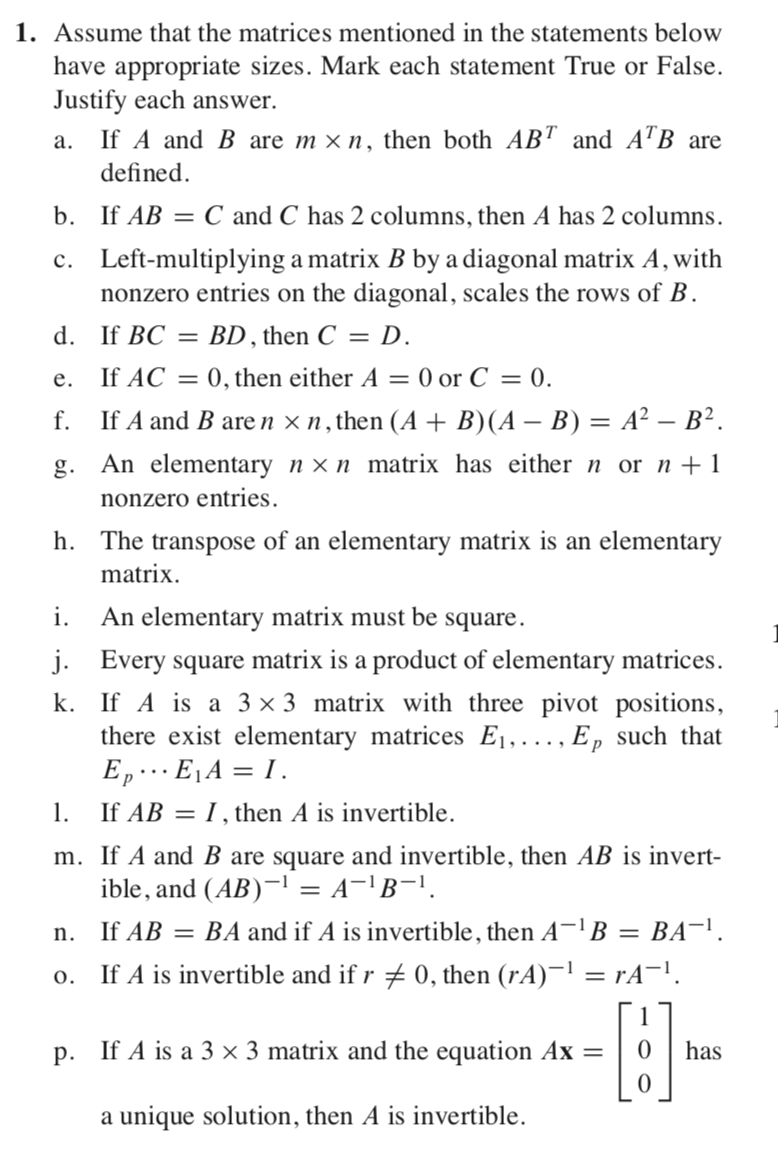
\includegraphics{Exam2TFa.png}
		\end{center}
		
		\newpage
			
		\item Practice True/False questions by doing problems 1(a)--1(p) from the below \ul{except} for parts \mbox{(f)--(h)} and part \mbox{(l)}:
		
		\begin{center}
			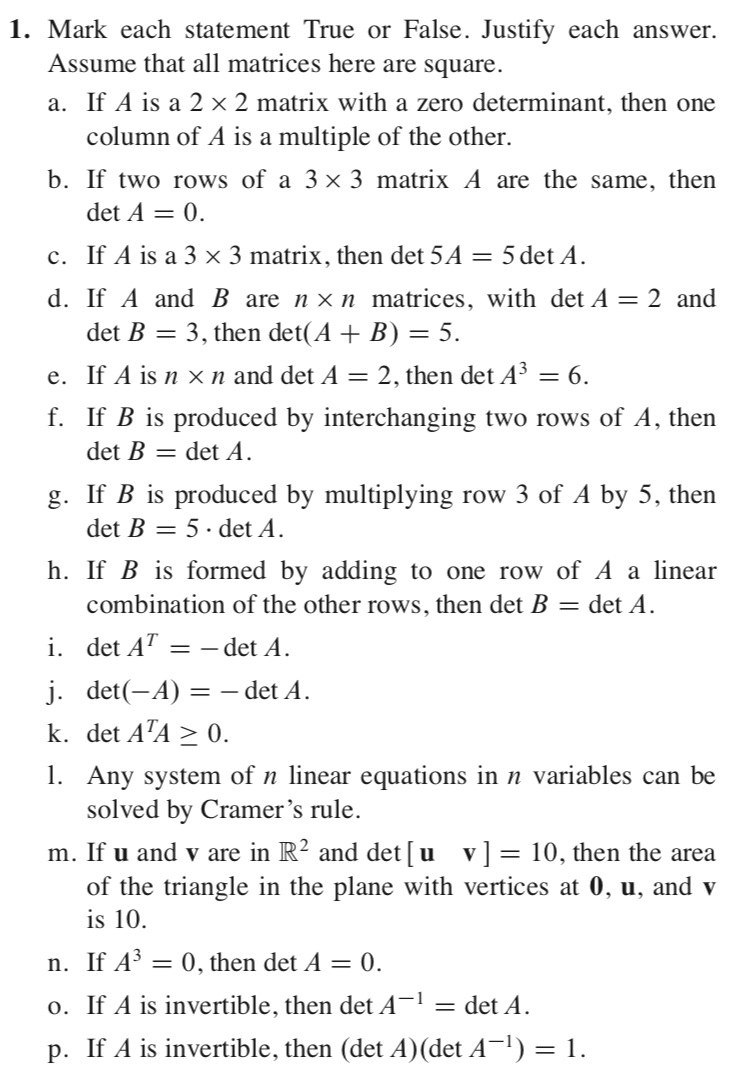
\includegraphics{Exam2TFb.png}
		\end{center}
	\end{enumerate}
\end{document}